% Bài báo ngắn 2 cột (6-8 trang) nộp vòng sơ loại — dịch bằng tectonic:  make paper-pdf
% Mọi số liệu lấy từ docs/competition-claims.md và docs/results.md (đã kiểm); số công suất: docs/energy-2026-10-29/.
\documentclass[11pt,a4paper,twocolumn]{article}
\usepackage{fontspec}
\setmainfont{Liberation Serif}
\setsansfont{Liberation Sans}
\setmonofont{DejaVu Sans Mono}[Scale=0.85]
\usepackage{polyglossia}
\setmainlanguage{vietnamese}
\usepackage[a4paper,top=17mm,bottom=17mm,left=16mm,right=16mm,columnsep=7mm]{geometry}
\usepackage{amsmath,amssymb}
\usepackage{booktabs,array}
\usepackage{graphicx}
\usepackage{caption}
\usepackage{enumitem}
\usepackage{xcolor}
\usepackage{tikz}
\usetikzlibrary{arrows.meta,positioning}
\usepackage{pgfplots}
\pgfplotsset{compat=1.17}
\usepackage{titlesec}
\usepackage[hidelinks,pdftitle={Edge AI Smart Laboratory Safety Monitoring System},pdfauthor={Lê Tự Thiện An; Trịnh Anh Văn; Võ Nhật Nam; Phạm Trọng Thành}]{hyperref}
\sloppy
\setlength{\parindent}{1.1em}
\setlength{\parskip}{0pt}
\captionsetup{font=small,labelfont=bf,labelsep=period,skip=3pt}
\setlist{itemsep=0pt,topsep=2pt,parsep=0pt,leftmargin=1.3em}
\titleformat{\section}{\normalfont\large\bfseries}{\thesection.}{0.5em}{}
\titleformat{\subsection}{\normalfont\normalsize\bfseries}{\thesubsection}{0.5em}{}
\titlespacing*{\section}{0pt}{7pt}{3pt}
\titlespacing*{\subsection}{0pt}{5pt}{2pt}
\renewcommand{\arraystretch}{1.1}
\definecolor{navy}{HTML}{16324F}
\definecolor{teal}{HTML}{0E7C86}
\definecolor{okg}{HTML}{2E9E4F}
\definecolor{crit}{HTML}{C62828}
\definecolor{mute}{HTML}{6B7280}
\newcommand{\file}[1]{\texttt{\small #1}}


\pgfplotsset{
  ch/.style={ybar,width=\linewidth,height=40mm,bar width=6mm,ymin=0,enlarge x limits=0.25,bar shift=0pt,
    /pgf/number format/use comma,
    tick label style={font=\fontsize{6.5}{8}\selectfont},label style={font=\fontsize{7}{8}\selectfont},
    title style={font=\fontsize{7.5}{9}\selectfont\bfseries,yshift=-1pt},
    nodes near coords,nodes near coords style={font=\fontsize{6.5}{8}\selectfont,text=black},
    ymajorgrids,grid style={gray!25},axis line style={gray!70}}}

\begin{document}

\twocolumn[{%
\begin{center}
{\LARGE\bfseries Edge AI Smart Laboratory Safety Monitoring System}\\[2mm]
{\large\bfseries Hệ thống AI biên giám sát an toàn phòng thí nghiệm theo thời gian thực\\
trên NPU RK3588S: lượng tử hóa INT8 và chế độ thích nghi}\\[3mm]
{\large
\textbf{Lê Tự Thiện An} (nhóm trưởng)\quad
Trịnh Anh Văn\\[0.5mm]
Võ Nhật Nam\quad
Phạm Trọng Thành}\\[1.5mm]
{\small Khoa Điện -- Điện tử, Trường Đại học Công nghệ Kỹ thuật TP. Hồ Chí Minh\\
EDGE AI DESIGN CHALLENGE 2026 -- Vòng sơ loại, tháng 11 năm 2026}
\end{center}
\vspace{1mm}
\begin{center}\begin{minipage}{0.92\textwidth}
\small\textbf{Tóm tắt.}
Bài báo trình bày một hệ thống giám sát an toàn phòng thí nghiệm chạy trên bo mạch Orange Pi 5 (RK3588S, NPU 6\,TOPS) với một camera USB.
Mô hình YOLO26n được lượng tử hóa INT8 để phát hiện người và áo blouse trên NPU. Khi một người không mặc áo blouse đứng trong vùng nguy hiểm do người dùng vẽ,
hệ thống cảnh báo trên trang web kèm ảnh bằng chứng, trên đèn LED, màn OLED và qua tin nhắn Zalo. Việc phát hiện và cảnh báo được thực hiện hoàn toàn tại chỗ;
Internet chỉ cần cho tin nhắn Zalo. Nhóm đề xuất cách xuất mô hình INT8 với đầu ra tách, giúp mAP50--95 chỉ giảm 0,4 điểm thay vì 18 điểm như cách xuất mặc định,
và chế độ chạy thích nghi giúp công suất bo mạch giảm từ 3,34\,W xuống 1,98\,W so với chế độ song song ở cùng tốc độ khung hình. Một bước kiểm tra tương đương
giữa đầu ra của NPU và CPU đã phát hiện bốn lỗi chuyển đổi mà các chỉ số tốc độ không phản ánh. Trên video phát lại, hệ thống đạt 29 khung hình/giây (25,9 khi bật
trang web), độ trễ p99 là 41,4\,ms và chạy ổn định trong 24 giờ. Khi đánh giá theo từng người trên ảnh kiểm tra, luật cảnh báo phát hiện được 75--86\% người không
mặc áo với tỉ lệ báo nhầm 7--9\%. Bài báo cũng ghi nhận một rủi ro khi triển khai: ở góc camera khác nhiều so với dữ liệu huấn luyện, mô hình không nhận ra áo
blouse ở khung hình nào.\\[1mm]
\textbf{Từ khóa:} edge AI, NPU, lượng tử hóa INT8, YOLO, an toàn phòng thí nghiệm, lập lịch thích nghi.
\end{minipage}\end{center}
\vspace{2mm}
}]

% ======================================================================
\section{Giới thiệu}

Trong phòng thí nghiệm hóa -- sinh, áo blouse là lớp bảo hộ cơ bản nhất. Việc nhắc nhở bằng người khó duy trì liên tục, trong khi gửi video lên máy chủ đám mây
vừa tốn băng thông vừa làm lộ hình ảnh của người trong phòng. Vì vậy, nhóm hướng tới một thiết bị đặt tại chỗ, tự xử lý hình ảnh và đáp ứng ba yêu cầu: chạy trên một bo mạch
giá thành thấp mà không phụ thuộc máy chủ; xử lý kịp tốc độ camera 30 khung hình/giây; và cảnh báo đúng đối tượng là người không mặc áo blouse đứng trong vùng nguy hiểm,
với vùng có thể vẽ lại khi thay đổi vị trí camera.

Bài toán kỹ thuật đặt ra là phân bổ các tác vụ lên các khối tính toán của RK3588S (4 nhân Cortex-A76, 4 nhân Cortex-A55 và NPU 3 nhân) sao cho hệ thống vẫn theo kịp
camera nhưng tốn ít tài nguyên và điện năng nhất. Các đóng góp chính của bài báo gồm:

\begin{enumerate}
  \item Một bước kiểm tra tương đương đầu ra giữa NPU và CPU, qua đó phát hiện bốn lỗi chuyển đổi mô hình mà tốc độ hay số lượng phát hiện không cho thấy (mục~\ref{sec:parity}).
  \item Cách xuất mô hình INT8 với đầu ra tách thành sáu tensor, giảm mức sụt mAP50--95 từ 18 điểm xuống 0,4 điểm (mục~\ref{sec:int8}).
  \item Chế độ chạy thích nghi, trong đó mô hình phụ chỉ được gọi khi cần và chạy bất đồng bộ trên nhân NPU riêng. So với chế độ song song, thời gian dùng NPU giảm 2,3 lần và công suất giảm 41\% (mục~\ref{sec:adapt}).
  \item Luật cảnh báo dựa trên điểm chân của người, chỉ kết luận vi phạm khi trang phục được nhìn thấy đủ rõ, kết hợp theo vết đối tượng và bước xác nhận theo thời gian (mục~\ref{sec:rule}).
  \item Quy trình chuẩn bị dữ liệu với ít nhãn và phần đánh giá ảnh hưởng của góc camera (mục~\ref{sec:data} và \ref{sec:angle}).
\end{enumerate}

Bảng~\ref{tab:req} đối chiếu các yêu cầu ban đầu với kết quả đạt được; các mục sau trình bày cách đo từng kết quả.

\begin{table}[t]
\centering
\caption{Yêu cầu đặt ra và kết quả đạt được.}
\label{tab:req}
\footnotesize
\begin{tabular}{@{}>{\raggedright\arraybackslash}p{2.9cm}>{\raggedright\arraybackslash}p{4.9cm}@{}}
\toprule
Yêu cầu & Kết quả \\
\midrule
Chạy tại chỗ, không phụ thuộc máy chủ & Toàn bộ suy luận trên NPU của bo mạch; chỉ tin Zalo cần Internet \\
Theo kịp camera 30 khung/giây & \textbf{29,02} khung/giây toàn hệ thống (video phát lại); 25,9 khi bật trang web \\
Độ trễ một khung dưới 50\,ms & p99 \textbf{41,4\,ms}; riêng tầng A p50 25,9\,ms \\
Cảnh báo đúng người, đúng vùng & Phát hiện 75--86\% người không mặc áo, báo nhầm 7--9\% (theo từng người); 97\% cùng quyết định trong/ngoài vùng \\
Tiết kiệm điện & \textbf{2,2\,W} khi chạy (0,86\,W khi nghỉ); chế độ thích nghi giảm 41\% so với chế độ song song \\
Hoạt động ổn định & Chạy liên tục 24 giờ, RAM 210--220\,MB, không lỗi \\
\bottomrule
\end{tabular}
\end{table}

% ======================================================================
\section{Công trình liên quan}

Phát hiện thiết bị bảo hộ cá nhân bằng học sâu đã được nghiên cứu nhiều, tiêu biểu là các hệ thống phát hiện mũ và áo bảo hộ trên công trường dùng mạng phát hiện một giai đoạn
họ YOLO \cite{nath,yolov1}. Các hệ thống này thường chạy trên máy chủ có GPU. Xu hướng edge AI đưa việc suy luận về thiết bị đầu cuối nhằm giảm độ trễ, băng thông và rủi ro lộ dữ liệu
\cite{chen}, trong đó lượng tử hóa số nguyên là kỹ thuật phổ biến để mô hình chạy nhanh trên NPU \cite{jacob}. Với bài toán theo vết, các phương pháp dựa trên IoU như SORT \cite{sort}
đủ hiệu quả trong cảnh ít người; hệ thống của nhóm dùng cách ghép tương tự và bổ sung ghép theo khoảng cách tâm.

Điểm khác biệt của bài báo không nằm ở việc sử dụng YOLO hay lượng tử hóa INT8, mà ở những vấn đề chỉ xuất hiện khi đưa toàn bộ hệ thống lên phần cứng thật. Chẳng hạn, công cụ
chuyển đổi mặc định cho ra mô hình INT8 chạy nhanh nhưng mất 18 điểm mAP50--95 mà không có cảnh báo nào. Lỗi này chỉ lộ ra khi đánh giá lại mô hình INT8 ngay trên NPU và chỉ khắc
phục được bằng cách thay đổi cấu trúc đầu ra. Tương tự, lợi ích của chế độ thích nghi chỉ đo đúng được khi cố định xung nhịp bộ nhớ và đo công suất bằng thiết bị đo.

% ======================================================================
\section{Hệ thống đề xuất}

Thiết kế của hệ thống có bốn ưu điểm chính. Thứ nhất, hệ thống xử lý hình ảnh hoàn toàn trên bo mạch nên không gửi hình người ra ngoài và vẫn hoạt động khi mất mạng. Thứ hai, hệ thống ưu tiên
độ tin cậy khi không chắc chắn: không báo AN TOÀN khi mất hình và không kết luận vi phạm khi chưa thấy rõ trang phục. Thứ ba, hệ thống tiêu thụ ít điện (2,2\,W) và có chế độ thích nghi để giảm tải khi
cần thêm tác vụ. Thứ tư, hệ thống dễ triển khai: vùng nguy hiểm được vẽ ngay trên trang web, cấu hình đổi được bằng một lệnh và các tầng xử lý có thể bật tắt độc lập.

\subsection{Phần cứng và luồng xử lý}

Phần cứng gồm bo mạch Orange Pi 5 (RK3588S, 8\,GB RAM), camera Logitech C270 ở độ phân giải $640{\times}480$ và 30 khung hình/giây, ba đèn LED và một màn hình OLED
$128{\times}64$ giao tiếp I2C, tất cả đặt trong vỏ in 3D (Hình~\ref{fig:hw}). Mô hình được chuyển đổi trên máy tính x86 bằng RKNN-Toolkit2 \cite{rknn} và chạy trên bo mạch bằng
thư viện \texttt{librknnrt} 2.3.2.

Hình~\ref{fig:pipe} mô tả luồng xử lý. Tầng A dùng YOLO26n \cite{yolo} với hai lớp \texttt{person} và \texttt{lab\_coat}, chạy trên mọi khung hình ở lõi NPU 0. Kết quả được đưa qua
bộ theo vết, bước gán áo cho từng người, luật vùng và bước xác nhận theo thời gian trước khi tới các đầu ra; Hình~\ref{fig:real} minh họa từng bước trên một khung hình thật.
Tầng B (kiểm tra thuộc tính trên ảnh cắt của từng người) và tầng C (phát hiện lửa, khói với tần suất 1\,Hz) chạy bất đồng bộ trên lõi NPU 1 và 2. Hai tầng này chỉ được dùng làm
tải thử nghiệm khi đánh giá chế độ thích nghi và được tắt trong sản phẩm vì chưa có dữ liệu thực tế. Chức năng phát hiện té ngã cũng đang tắt.

\begin{figure}[t]
\centering
\begin{tikzpicture}[
  bx/.style={draw=navy,line width=0.6pt,rounded corners=1.5pt,fill=white,align=center,minimum height=7.5mm,minimum width=25mm,font=\fontsize{6.5}{7.5}\selectfont,inner sep=2pt},
  hl/.style={bx,fill=teal!14},
  as/.style={bx,dash pattern=on 2pt off 1.5pt,minimum width=25mm},
  ar/.style={-{Stealth[length=1.8mm]},line width=0.6pt,draw=navy},
  da/.style={-{Stealth[length=1.8mm]},line width=0.6pt,draw=navy,dash pattern=on 2pt off 1.5pt}]
  \node[bx] (c) at (0,0) {Camera USB\\30 FPS};
  \node[hl,right=4mm of c] (a) {\textbf{Tầng A}: YOLO26n\\INT8, NPU lõi 0};
  \node[bx,right=4mm of a] (t) {Theo vết người\\+ gán áo};
  \node[hl,below=5mm of t] (z) {\textbf{Luật vùng}\\chân trong đa giác};
  \node[bx,left=4mm of z] (d) {Xác nhận 3 s\\nghỉ 60 s};
  \node[hl,left=4mm of d] (o) {\textbf{Đầu ra}: web, LED,\\OLED, Zalo};
  \node[as,above=4.5mm of a] (b) {Tầng B (thử), lõi 1};
  \node[as,left=4mm of b] (cc) {Tầng C (thử), lõi 2};
  \draw[ar](c)--(a);\draw[ar](a)--(t);\draw[ar](t)--(z);\draw[ar](z)--(d);\draw[ar](d)--(o);
  \draw[da](a)--(b);\draw[da](c.north)--++(0,3mm)-|(cc.south);
\end{tikzpicture}
\caption{Luồng xử lý. Nét liền: chạy trên mọi khung hình. Nét đứt: chạy bất đồng bộ, chỉ dùng khi đánh giá chế độ thích nghi.}
\label{fig:pipe}
\end{figure}

\begin{figure}[t]
\centering
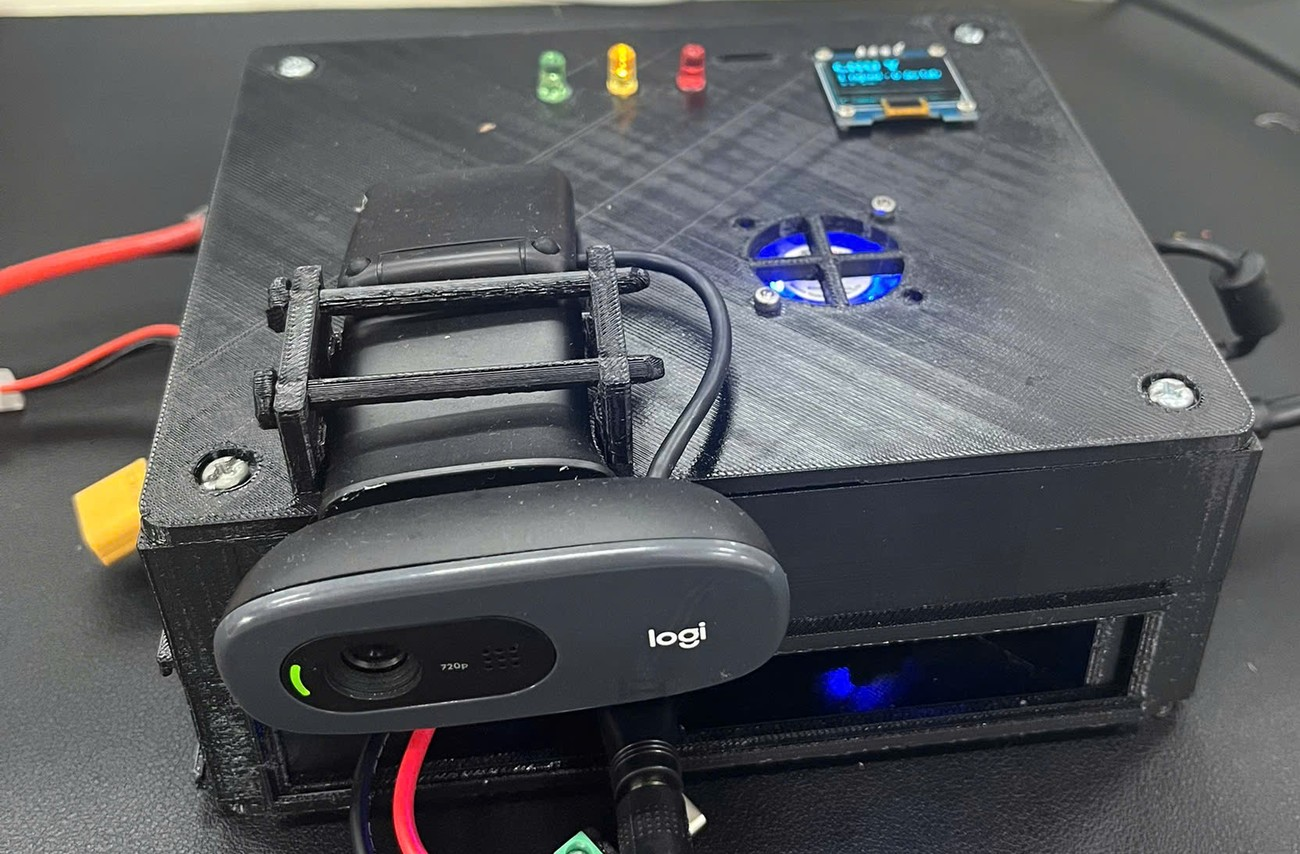
\includegraphics[width=0.86\columnwidth]{../poster/img/hardware_full.jpg}
\caption{Sản phẩm hoàn chỉnh: Orange Pi 5 trong vỏ in 3D, camera C270, ba đèn LED (xanh, vàng, đỏ), màn OLED và quạt tản nhiệt.}
\label{fig:hw}
\end{figure}

\subsection{Quy tắc cảnh báo}
\label{sec:rule}

Để xác định một người có ở trong vùng nguy hiểm hay không, hệ thống dùng \emph{điểm chân} của người đó, tức trung điểm cạnh dưới khung bao
$p=\big(\tfrac{x_1+x_2}{2},\,y_2\big)$, thay vì tâm khung. Lý do là với một người đứng ngay phía sau vùng, tâm khung có thể rơi vào trong vùng dù người đó chưa bước vào
(Hình~\ref{fig:foot}). Người được xem là ở trong vùng $Z$ khi $p\in Z$, kiểm tra bằng thuật toán tia trên đa giác đã chuẩn hóa về $[0,1]^2$.
Một người được xem là đang mặc áo nếu trong 2\,s gần nhất có một khung áo $g$ thỏa mãn
\begin{equation}
  \frac{|g\cap d|}{|g|}\ge 0{,}5\quad\text{và}\quad \operatorname{conf}(g)\ge\tau=0{,}6,
\end{equation}
trong đó $d$ là khung của người. Mỗi khung áo chỉ được gán cho đúng một người có tỉ lệ chứa lớn nhất, nhằm tránh gán nhầm áo giữa hai người đứng sát nhau.
Ngưỡng $\tau$ của áo được đặt cao hơn ngưỡng của người, vì một khung áo sai sẽ khiến người vi phạm không bị cảnh báo, và đây là loại sai nguy hiểm hơn báo nhầm.

\begin{figure}[t]
\centering
\begin{tikzpicture}[x=1mm,y=1mm,font=\fontsize{6.5}{7.5}\selectfont]
  \fill[violet!18,draw=violet!70,line width=0.7pt] (2,2) -- (62,2) -- (74,28) -- (8,28) -- cycle;
  \node[violet!70!black] at (38,23.5) {vùng nguy hiểm (vẽ trên sàn)};
  % A: chân trong vùng, có áo
  \draw[orange!85!black,line width=0.8pt] (12,6) rectangle (22,34);
  \draw[okg,line width=0.5pt] (13,16) rectangle (21,30);
  \fill[orange!85!black] (17,6) circle (1.1);
  \node[align=center] at (17,-3) {A: chân trong,\\có áo $\Rightarrow$ không báo};
  % B: chân trong, không áo
  \draw[crit,line width=0.8pt] (34,6) rectangle (45,34);
  \fill[crit] (39.5,6) circle (1.1);
  \node[align=center] at (40,-3) {B: chân trong,\\không áo $\Rightarrow$ \textbf{báo động}};
  % C: thân che lên vùng nhưng chân ngoài
  \draw[gray,line width=0.8pt] (58,30) rectangle (69,56);
  \fill[gray] (63.5,30) circle (1.1);
  \node[align=center] at (63,60) {C: chân ngoài\\$\Rightarrow$ chưa vào vùng};
\end{tikzpicture}
\caption{Quy tắc điểm chân (chấm tròn). Chỉ điểm chân được dùng để xét vùng; việc có mặc áo hay không được xác định ở bước riêng (khung xanh mỏng là khung áo). Thân người C che lên vùng nhưng chân nằm ngoài nên chưa được tính là vào vùng.}
\label{fig:foot}
\end{figure}

Một người bị xem là vi phạm khi đồng thời có chân trong vùng, không mặc áo và trang phục được nhìn thấy đủ rõ. Điều kiện cuối là cần thiết vì không thấy áo chưa chắc là
không mặc áo. Những người chỉ lộ mặt ở mép khung hình, bị người gần camera hơn che quá 40\% khung, hoặc có khung quá nhỏ sẽ được đánh dấu là \emph{chưa thấy rõ áo} và không bị
tính là vi phạm. Trên một video quay ở phòng thí nghiệm đông người dài 170\,s, quy tắc này giảm số cảnh báo từ 31 xuống 6, và cả 6 cảnh báo còn lại đều đúng.

Cảnh báo chỉ được phát khi vi phạm kéo dài liên tục 3\,s, có cho phép gián đoạn tối đa 1\,s để một khung hình bị bỏ sót không làm mất thời gian đã tích lũy. Sau khi cảnh báo,
hệ thống không báo lại cùng một người trong 60\,s. Bộ theo vết ghép khung giữa các khung hình liên tiếp theo IoU $\ge0{,}3$, sau đó theo khoảng cách tâm, và giữ mã của người mất dấu
tối đa 3\,s. Với thời gian giữ 1,5\,s, một buổi chạy 15 phút đã sinh ra 24 mã cho chỉ 2--4 người, mỗi mã mới tương ứng với một cảnh báo thừa.

\begin{figure}[t]
\centering
\fbox{\parbox{0.93\columnwidth}{\footnotesize\textbf{Thuật toán 1.} Một vòng lặp xử lý (chế độ thích nghi).
\begin{enumerate}[leftmargin=1.4em,itemsep=0pt,topsep=1pt]
\item Chờ \emph{ảnh mới} từ camera (không đọc lặp ảnh cũ).
\item Tầng A (NPU lõi 0) $\to$ khung người và khung áo.
\item Bộ theo vết cập nhật mã người; gán mỗi khung áo cho một người (tỉ lệ chứa $\ge0{,}5$, $\mathrm{conf}\ge\tau$).
\item Mỗi người: nếu chân $\in Z$ $\wedge$ không mặc áo $\wedge$ thấy rõ trang phục thì ghi nhận vi phạm.
\item Người nào đến hạn kiểm tra (2\,s): gửi ảnh cắt cho tầng B (lõi 1), \emph{không chờ}; mỗi 1\,s gửi khung cho tầng C (lõi 2), không chờ.
\item Xác nhận: vi phạm kéo dài $\ge3$\,s (cho phép gián đoạn 1\,s) $\Rightarrow$ báo động, sau đó không báo lại người đó trong 60\,s.
\item Cập nhật trang, LED, OLED; nếu quá 3\,s không có khung mới thì hiện MẤT TÍN HIỆU.
\end{enumerate}}}
\label{alg:loop}
\end{figure}

\begin{figure*}[t]
\centering
\begin{minipage}{0.43\textwidth}\centering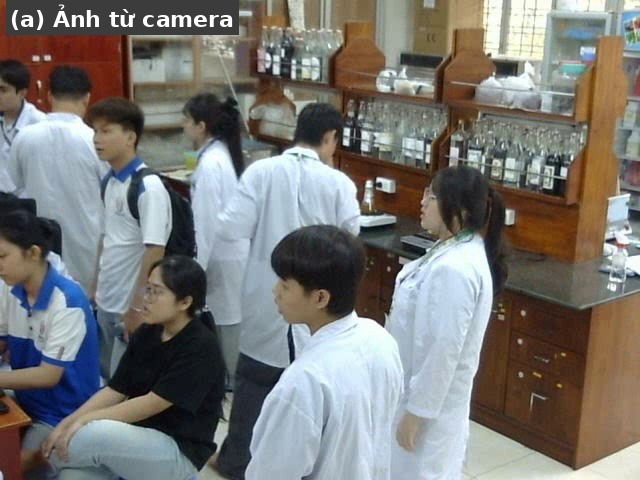
\includegraphics[width=\linewidth]{img/pipe_a.jpg}\end{minipage}\hspace{2mm}
\begin{minipage}{0.43\textwidth}\centering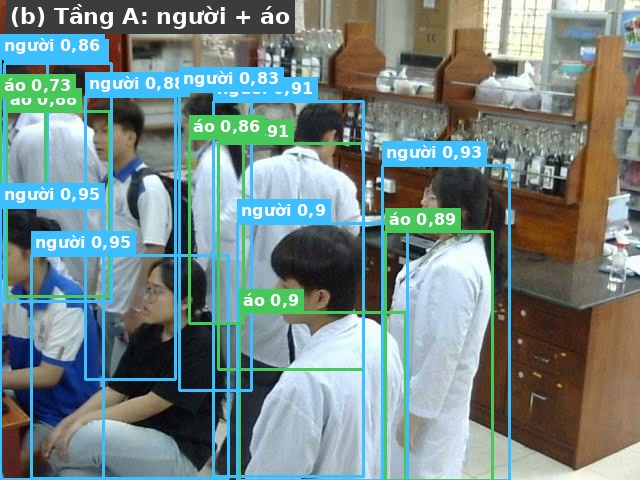
\includegraphics[width=\linewidth]{img/pipe_b.jpg}\end{minipage}\\[1mm]
\begin{minipage}{0.43\textwidth}\centering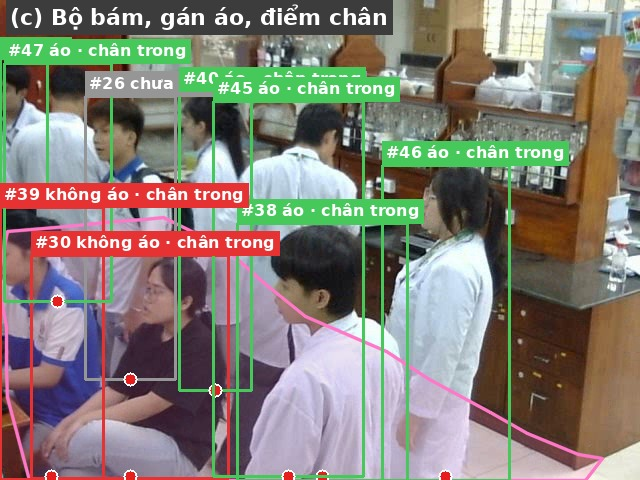
\includegraphics[width=\linewidth]{img/pipe_c.jpg}\end{minipage}\hspace{2mm}
\begin{minipage}{0.43\textwidth}\centering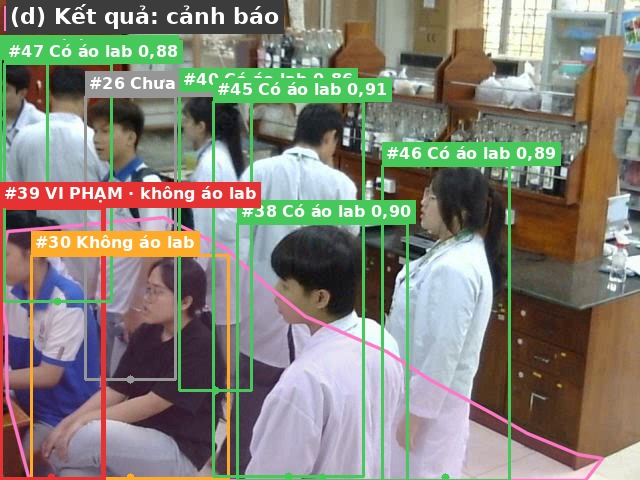
\includegraphics[width=\linewidth]{img/pipe_d.jpg}\end{minipage}
\caption{Luồng xử lý trên một khung hình thật từ video quay tại phòng thí nghiệm; các khung và nhãn do chính phần mềm của hệ thống vẽ. (a) Ảnh từ camera. (b) Đầu ra tầng A:
khung người (xanh dương) và khung áo (xanh lá) kèm độ tin cậy. (c) Bộ theo vết gán mã cho từng người, gán khung áo cho người và đánh dấu điểm chân (chấm tròn, màu đỏ khi chân nằm
trong vùng tím); người chưa thấy rõ áo (xám) không bị xét vi phạm. (d) Kết quả: người không mặc áo, có chân trong vùng và đã vi phạm đủ 3\,s được đánh dấu VI PHẠM (đỏ); người không mặc
áo đang chờ xác nhận hoặc ở ngoài vùng có màu cam.}
\label{fig:real}
\end{figure*}

\subsection{Đầu ra và giao diện}

Trang web, đèn và màn OLED dùng chung bốn trạng thái (Bảng~\ref{tab:states}; giao diện thực tế ở Hình~\ref{fig:ui}). Nguyên tắc thiết kế là không bao giờ hiển thị
AN TOÀN khi hệ thống không nhận được hình. Trang web bằng tiếng Việt, được truy cập qua đường hầm SSH thay vì mở ra mạng, gồm video có vẽ khung, số người trong vùng, biểu đồ 15 phút
gần nhất và lịch sử cảnh báo kèm ảnh cắt của người vi phạm. Khi đổi vị trí camera, người dùng vẽ lại vùng nguy hiểm trực tiếp trên video; vùng mới được kiểm tra hợp lệ (đa giác không
tự cắt, tọa độ trong $[0,1]$) trước khi áp dụng.

Mỗi cảnh báo cũng được gửi thành một tin nhắn Zalo, các cảnh báo trong cùng 10\,s được gộp thành một tin. Đây là phần duy nhất cần Internet. Ảnh của người vi phạm không được gửi
qua Zalo vì Zalo chỉ nhận ảnh qua đường dẫn công khai; người phụ trách xem ảnh trên trang web. Bảng~\ref{tab:feat} liệt kê các tính năng của sản phẩm và mức kiểm chứng của từng tính năng.

\begin{table}[t]
\centering
\caption{Tính năng của sản phẩm và mức kiểm chứng.}
\label{tab:feat}
\footnotesize
\begin{tabular}{@{}>{\raggedright\arraybackslash}p{2.4cm}>{\raggedright\arraybackslash}p{3.6cm}>{\raggedright\arraybackslash}p{1.8cm}@{}}
\toprule
Tính năng & Mô tả & Mức kiểm chứng \\
\midrule
Phát hiện người và áo blouse & YOLO26n INT8 trên NPU, 29 khung/giây & Đo trên bo mạch \\
Vùng nguy hiểm tự vẽ & Vẽ, lưu, khôi phục ngay trên trang web; kiểm tra hợp lệ trước khi áp dụng & Chạy thử \\
Ảnh bằng chứng & Ảnh người vi phạm và toàn khung hình, lịch sử cảnh báo, biểu đồ 15 phút & Chạy thử \\
Đèn LED, màn OLED & Bốn trạng thái; OLED hiển thị số người vi phạm & Đã kiểm tra từng trạng thái \\
Tin nhắn Zalo & Tin chữ, gộp các cảnh báo trong 10\,s; cần Internet & Đã nhận tin thật \\
Chạy tự động & Tự khởi động khi cấp nguồn, tự phục hồi khi mất camera & Đo 24 giờ \\
Té ngã, lửa và khói & Đã có mã nguồn nhưng đang tắt & Chưa đánh giá \\
\bottomrule
\end{tabular}
\end{table}

\begin{table}[t]
\centering
\caption{Bốn trạng thái của hệ thống.}
\label{tab:states}
\footnotesize
\begin{tabular}{@{}>{\raggedright\arraybackslash}p{2.2cm}>{\raggedright\arraybackslash}p{3.6cm}>{\raggedright\arraybackslash}p{2.0cm}@{}}
\toprule
Trạng thái & Điều kiện & Đèn / OLED \\
\midrule
AN TOÀN & có hình, không vi phạm & xanh \\
CHÚ Ý & có người không mặc áo ngoài vùng, vi phạm đang chờ xác nhận, hoặc vừa có cảnh báo (10\,s) & vàng \\
BÁO ĐỘNG & không mặc áo, ở trong vùng, kéo dài 3\,s & đỏ nháy, OLED nháy \\
MẤT TÍN HIỆU & không có khung mới quá 3\,s & vàng nháy chậm \\
\bottomrule
\end{tabular}
\end{table}

\begin{figure*}[t]
\centering
\begin{minipage}[t]{0.60\textwidth}\centering\vspace{0pt}
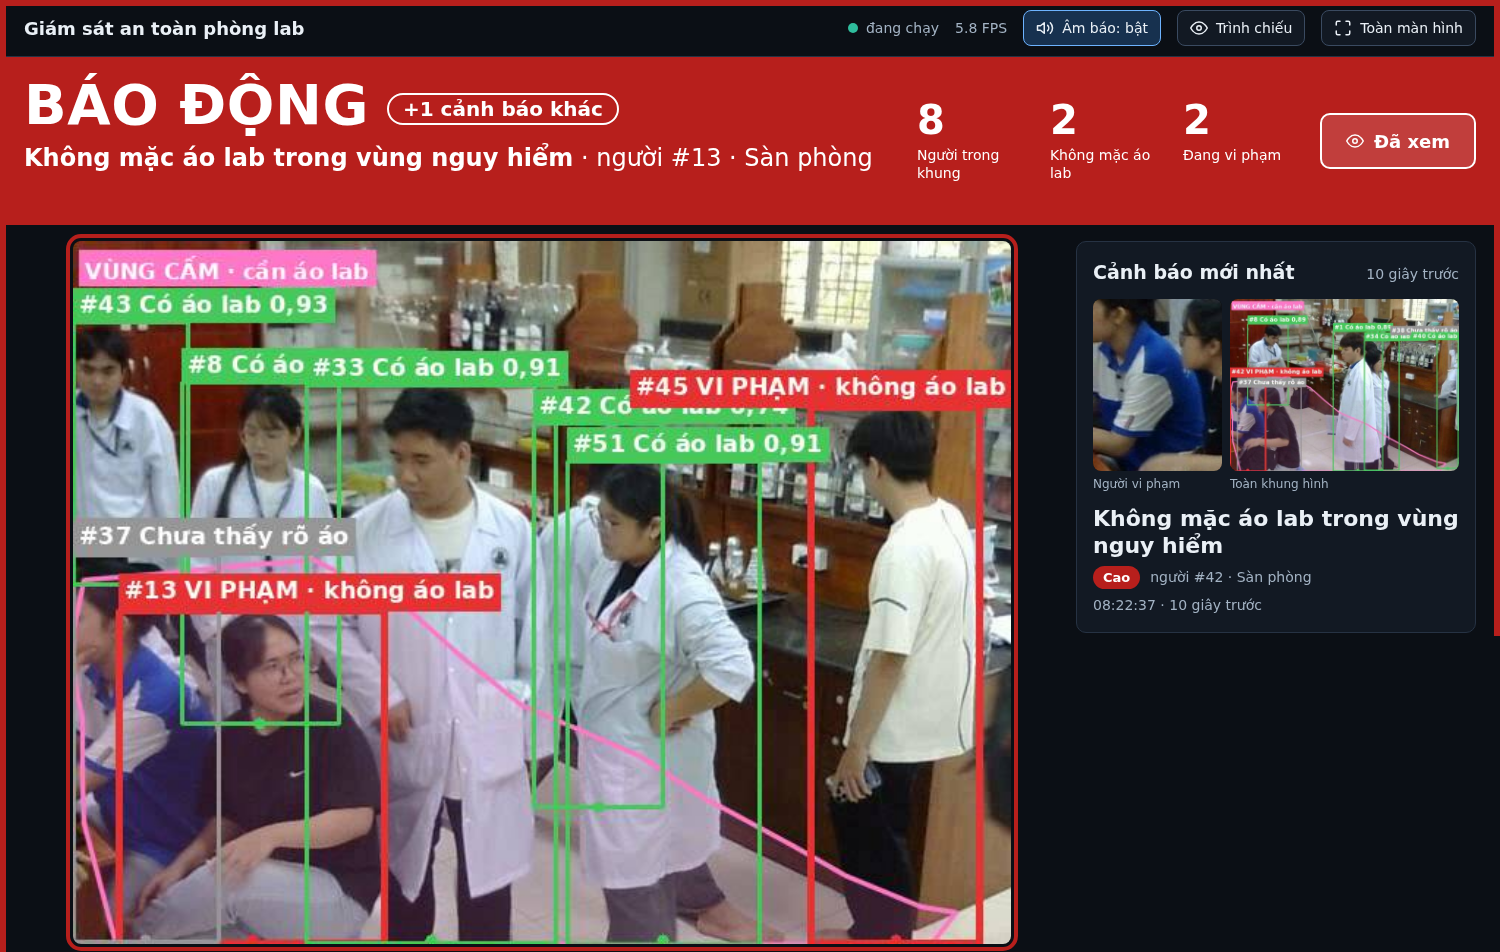
\includegraphics[width=\linewidth]{img/dashboard.png}
\end{minipage}\hfill
\begin{minipage}[t]{0.31\textwidth}\centering\vspace{0pt}
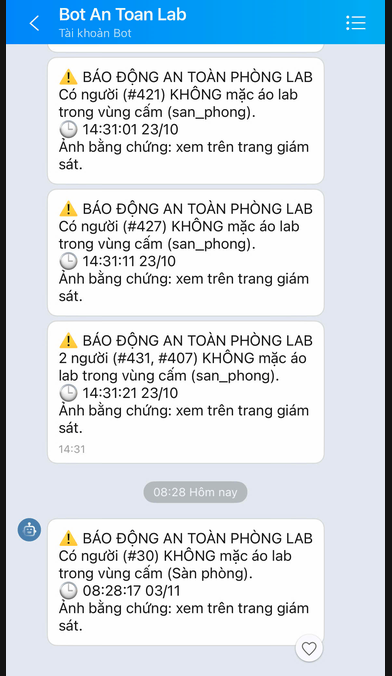
\includegraphics[width=\linewidth]{img/zalo.png}
\end{minipage}
\caption{Giao diện và tin nhắn thực tế. Trái: trang web giám sát khi có báo động, gồm thanh trạng thái, số người, video có khung và ảnh của cảnh báo mới nhất. Ảnh được chụp khi chạy
thử trên máy tính với video quay ở phòng thí nghiệm, nên tốc độ hiển thị không phải của bo mạch. Phải: tin nhắn Zalo nhận trên điện thoại; ba tin ngày 23/10 phát sinh trong lần chạy thử,
tin ngày 03/11 được gửi bằng chính mô-đun gửi tin của hệ thống.}
\label{fig:ui}
\end{figure*}

\subsection{Triển khai và vận hành}

Phần mềm chạy dưới dạng dịch vụ \texttt{systemd}: tự khởi động khi cấp nguồn và tự khởi động lại sau 10\,s nếu gặp lỗi, kể cả khi lúc bật máy chưa cắm camera. Dịch vụ bị giới hạn
1,5\,GB RAM để một lỗi rò bộ nhớ không ảnh hưởng tới cả bo mạch, và được dừng bằng tín hiệu cho phép đóng tệp an toàn. Do bo mạch không có pin giữ giờ, đồng hồ được đồng bộ từ máy tính
mỗi lần khởi động, còn thời gian trên trang web được hiển thị theo đồng hồ của máy người xem. Khi camera bị rút, hệ thống tự thử kết nối lại và trang web chuyển sang MẤT TÍN HIỆU thay vì
báo an toàn.

% ======================================================================
\section{Tối ưu hóa và tăng tốc}

\subsection{Chuyển từ CPU sang NPU và kiểm tra tương đương}
\label{sec:parity}

Với cùng mô hình YOLO26n, thời gian xử lý một khung ở tầng A là 25,1\,ms trên NPU với INT8, so với 47,8\,ms ở FP16 và 90,9\,ms trên CPU với ONNX FP32 (Hình~\ref{fig:charts}a).
Khi chạy trên CPU, hệ thống chỉ đạt 10,5 khung hình/giây và nhiệt độ SoC lên tới 86,8\,$^\circ$C sau khoảng 2 phút. Do tốc độ tổng bị giới hạn bởi camera,
$\mathrm{FPS}=\min(f_{\text{cam}},1/T_{\text{khung}})$, nên khi $1/T_{\text{khung}}>30$, việc tăng tốc phần suy luận không làm tăng FPS mà chỉ giảm tải và nhiệt độ.

Việc chuyển mô hình sang NPU có thể gây lỗi mà không có dấu hiệu rõ ràng: mô hình vẫn chạy nhanh và vẫn cho ra phát hiện, nhưng kết quả sai. Nhóm đã gặp bốn lỗi như vậy, gồm
đầu ra end-to-end gây lỗi bộ nhớ, mô hình INT8 không phát hiện được gì, ảnh bị chuẩn hóa hai lần, và tọa độ INT8 bị chia cho kích thước ảnh (phiên bản đầu cho 49 phát hiện nhưng
không khớp phát hiện nào). Để chặn các lỗi này, nhóm thêm bước kiểm tra tương đương: cùng một tập ảnh được chạy qua bản ONNX và bản NPU, các khung được ghép theo IoU, sau đó tính
$R=\tfrac{TP}{TP+FN}$, $P=\tfrac{TP}{TP+FP}$ và $\overline{\mathrm{IoU}}=\tfrac{1}{TP}\sum_{(a,b)}\tfrac{|a\cap b|}{|a\cup b|}$ trên các cặp khung khớp. Ngoài ra, mỗi mô hình đi kèm
một tệp mô tả cách chuẩn hóa ảnh và dạng tọa độ đầu ra, và hệ thống từ chối nạp mô hình nếu thiếu tệp này.

\begin{table}[t]
\centering
\caption{Kết quả kiểm tra tương đương trên bo mạch (INT8 so với ONNX, ghép khung khi IoU $\ge0{,}5$).}
\label{tab:parity}
\footnotesize
\begin{tabular}{@{}lrrr@{}}
\toprule
Mô hình (số ảnh) & $R$ & $P$ & $\overline{\mathrm{IoU}}$ \\
\midrule
\texttt{lab\_v3}, INT8 một tensor (40) & 0,92 & 0,87 & 0,82 \\
\texttt{lab\_v6}, INT8 một tensor (78) & 0,98 & 0,93 & 0,84 \\
\texttt{lab\_v6}, \textbf{đầu ra tách} (99) & 0,98 & 1,00 & \textbf{0,97} \\
\bottomrule
\end{tabular}
\end{table}

\subsection{Lượng tử hóa INT8 với đầu ra tách}
\label{sec:int8}

Khi đánh giá lại mô hình INT8 chạy trên NPU bằng cùng bộ đánh giá với bản FP32, nhóm nhận thấy cách xuất mặc định làm mAP50--95 giảm 18 điểm. Nguyên nhân là đầu ra mặc định gộp
tọa độ khung và điểm lớp vào một tensor, dùng chung một thang lượng tử 8 bit \cite{jacob}. Bước lượng tử khi đó là $s=(r_{\max}-r_{\min})/255$; vì thang phải phủ cả tọa độ (khoảng
$[0,640]$ điểm ảnh) lẫn điểm lớp ($[0,1]$), $s\approx640/255\approx2{,}5$ điểm ảnh. Giá trị này cùng bậc với độ lệch 2,7 điểm ảnh đo được ở mép khung và làm IoU so với bản FP32 chỉ còn
0,84. Các cách thông thường như đổi thuật toán hiệu chuẩn sang KL, lượng tử hóa hỗn hợp hay thay bộ ảnh hiệu chuẩn đều không cải thiện được.

Nhóm giải quyết bằng cách xuất mô hình với sáu tensor đầu ra, gồm khung và điểm lớp riêng cho từng tầng đặc trưng, mỗi tensor có thang lượng tử riêng, rồi giải mã trên CPU với chi phí
không đáng kể. Như Bảng~\ref{tab:int8}, mAP50--95 khi đó chỉ giảm 0,4 điểm ở góc 1 (độ lệch chuẩn 0,004 qua 3 lần huấn luyện), và IoU trong bước kiểm tra tương đương tăng từ 0,84 lên 0,97.
Về độ phân giải đầu vào, 416 cho kết quả kém rõ rệt, còn 512 tương đương 640 về mAP50 nhưng kém hơn với người ở xa, nên hệ thống dùng 640.

\begin{table}[t]
\centering
\caption{Độ chính xác của mô hình sau lượng tử hóa trên tập kiểm tra độc lập ở góc 1. Ở góc 2, mAP50--95 lần lượt là 0,791, 0,590 và 0,784.}
\label{tab:int8}
\footnotesize
\begin{tabular}{@{}lrr@{}}
\toprule
Cấu hình & mAP50 & mAP50--95 \\
\midrule
FP32 & 0,864 & 0,661 \\
INT8 một tensor (mặc định) & 0,828 & 0,481 \\
\textbf{INT8 đầu ra tách} (TB 3 lần) & \textbf{0,869} & \textbf{0,657} \\
\bottomrule
\end{tabular}
\end{table}

\subsection{Chế độ thích nghi và điện năng}
\label{sec:adapt}

Ở chế độ song song, tầng B chạy cho mọi người và tầng C chạy trên mọi khung hình. Ở chế độ thích nghi, tầng B chỉ chạy cho người đến lượt kiểm tra lại (mỗi 2\,s) và tầng C chạy với tần
suất 1\,Hz. Cả hai tầng chạy trên lõi NPU riêng nên không làm tăng thời gian xử lý mỗi khung, nhờ đó độ trễ p99 giảm từ 61,2 xuống 49,9\,ms. Mỗi chế độ được đo 3 lượt, mỗi lượt 15 phút,
trên cùng một video 30 khung hình/giây. Công suất được đo bằng đồng hồ USB-C đặt giữa nguồn và bo mạch, đọc theo điện năng tích lũy (mWh), với sai số tuyệt đối khoảng $\pm10\%$. Trước khi
đo, đồng hồ đã được kiểm tra: ở tải thường, số đọc 3,54\,W khớp với tích $V\!\times\!A$, và khi cho CPU chạy hết công suất, số đọc tăng từ 3,2 lên 8,3\,W.

\begin{table}[t]
\centering
\caption{Chế độ thích nghi so với chế độ song song (video phát lại 30 khung hình/giây; công suất đo một lần mỗi chế độ).}
\label{tab:adapt}
\footnotesize
\begin{tabular}{@{}lrr@{}}
\toprule
 & Thích nghi & Song song \\
\midrule
Gọi tầng B / C mỗi khung & 0,07 / 0,03 & 3,1 / 1,0 \\
Thời gian NPU mỗi khung & \textbf{32\,ms} & 74\,ms \\
CPU của tiến trình & \textbf{35\%} & 73\% \\
Nhiệt độ SoC ổn định & \textbf{41,5\,$^\circ$C} & 54,3\,$^\circ$C \\
Công suất bo mạch (nghỉ 0,86\,W) & \textbf{1,98\,W} & 3,34\,W \\
Năng lượng mỗi khung & \textbf{69\,mJ} & 113\,mJ \\
FPS khi đo công suất & 28,9 & 29,7 \\
\bottomrule
\end{tabular}
\end{table}

Ở cùng tốc độ khoảng 29 khung hình/giây, chế độ thích nghi tiêu thụ ít hơn chế độ song song 1,36\,W, tức 41\%, và năng lượng cho mỗi khung giảm khoảng 39\% (Bảng~\ref{tab:adapt},
Hình~\ref{fig:charts}c). Đây là so sánh giữa hai chế độ của cùng một hệ thống. Cấu hình sản phẩm, chỉ dùng tầng A nhưng có thêm trang web, đèn LED và OLED, tiêu thụ 2,20\,W; mức chênh so với
chế độ thích nghi nằm trong sai số của đồng hồ nên nhóm không kết luận cấu hình nào tốn điện hơn.

Khi so sánh tốc độ cần chú ý một điểm: với cấu hình xung nhịp mặc định, lúc tải nhẹ bo mạch tự hạ xung bộ nhớ DDR từ 2112 xuống 528\,MHz, khiến chế độ thích nghi có vẻ chậm hơn
(28,2 so với 29,8 khung hình/giây). Vì vậy, khi so sánh hai chế độ có mức tải khác nhau cần cố định xung nhịp; nếu không, kết quả phản ánh bộ điều khiển xung nhịp chứ không phải thuật toán.

\subsection{Các tối ưu khác trong hệ thống}

Bảng~\ref{tab:opt} tổng hợp các tối ưu cùng số đo trước và sau khi áp dụng. Khi camera được đọc theo kiểu chờ ảnh mới thay vì đọc lặp, FPS giảm từ 37 xuống 29,6; con số 37 trước đó cao hơn
thực tế vì tính cả các lần xử lý lại ảnh cũ. Ngoài ra, mô hình nhỏ chưa chắc có chi phí thấp tương ứng: mỗi lần gọi một mô hình trên NPU có chi phí cố định khoảng 10\,ms, nên tầng B chỉ nhanh hơn
tầng A 2,4 lần dù ảnh đầu vào nhỏ hơn 4 lần. Việc cố định xung DDR trong dịch vụ triển khai giúp FPS toàn hệ thống tăng từ 26,84 lên 29,02, đổi lại nhiệt độ cuối tăng 3,1\,$^\circ$C.

\begin{table}[t]
\centering
\caption{Các tối ưu và số đo trước, sau khi áp dụng.}
\label{tab:opt}
\footnotesize
\begin{tabular}{@{}>{\raggedright\arraybackslash}p{3.0cm}>{\raggedright\arraybackslash}p{2.5cm}>{\raggedright\arraybackslash}p{2.5cm}@{}}
\toprule
Kỹ thuật & Trước & Sau \\
\midrule
Giải mã chỉ lớp cần giữ & 2,1\,ms & 0,38\,ms \\
Tầng B, C bất đồng bộ (mỗi tầng một nhân NPU) & p99 61,2\,ms & p99 49,9\,ms \\
Camera chờ ảnh mới & 37 FPS, đếm cả 20\% ảnh lặp & 29,6 FPS \\
Chống báo lặp (nghỉ 60\,s, giữ mã 3\,s) & 122 cảnh báo / 14,5 phút & 24 cảnh báo / 9,5 phút \\
Khóa xung DDR & 26,84 FPS, p99 44,1\,ms & 29,02 FPS, p99 41,4\,ms \\
INT8 đầu ra tách & mAP50--95 0,481 & 0,657 \\
\bottomrule
\end{tabular}
\end{table}

% ======================================================================
\section{Dữ liệu và huấn luyện}
\label{sec:data}

Dữ liệu được thu bằng cách cho bo mạch tự chụp một ảnh mỗi 4 giây tại phòng thí nghiệm, ở hai góc camera khác nhau. Khoảng 1\,700 ảnh đã được gán nhãn, phần lớn có 5--6 người mỗi ảnh,
với hai lớp \texttt{person} và \texttt{lab\_coat}. Các lớp kính và găng tay ban đầu đã bị loại vì dữ liệu cho thấy không ai đeo kính, còn găng tay chỉ xuất hiện dưới dạng một đôi đặt trên bàn.

Quy trình gán nhãn gồm các bước: chọn ra những ảnh khác nhau nhiều nhất bằng phương pháp lấy mẫu điểm xa nhất trên ảnh thu nhỏ $48{\times}36$, kết hợp với các ảnh mà mô hình còn phân vân về áo;
dùng mô hình hiện có tạo nhãn nháp để người gán nhãn chỉ cần xóa nhãn sai và bổ sung nhãn thiếu; huấn luyện 3 lần với 3 hạt giống ngẫu nhiên; và đánh giá trên một phiên thu khác (ngày khác,
người khác). Bảng~\ref{tab:data} tóm tắt tác dụng của từng bước.

\begin{table}[t]
\centering
\caption{Các bước trong quy trình dữ liệu và kết quả đo được.}
\label{tab:data}
\footnotesize
\begin{tabular}{@{}>{\raggedright\arraybackslash}p{3.4cm}>{\raggedright\arraybackslash}p{4.6cm}@{}}
\toprule
Bước & Kết quả \\
\midrule
Mô hình huấn luyện trên ảnh công trường, dùng trong lab & phát hiện người kém hơn mô hình gốc (16/20 so với 20/20 ảnh) \\
Dùng mô hình open-vocabulary để tự gán nhãn & AP50 với kính chỉ 0,13--0,20, không dùng được \\
\textbf{Chọn ảnh khó} & độ chính xác áo \textbf{0,52 $\to$ 0,76} \\
\textbf{Thêm 238 ảnh COCO âm tính} & áo thun trắng bị nhận nhầm là áo blouse: 20/20 $\to$ 0--4/20 ảnh \\
Mô hình lớn hơn (YOLO26s) & chỉ tốt hơn khoảng 2 điểm nhưng chậm hơn 2--3 lần \\
\bottomrule
\end{tabular}
\end{table}

Kết quả cho thấy việc chọn đúng ảnh khó mang lại nhiều cải thiện hơn việc dùng mô hình lớn hơn, tức điểm nghẽn nằm ở dữ liệu. Một lỗi đáng chú ý là mọi mô hình chỉ học từ ảnh trong
phòng thí nghiệm đều nhận nhầm \emph{áo thun trắng} là áo blouse ở 19--20 trên 20 ảnh kiểm tra, do trong phòng có quá ít người mặc áo trắng thông thường. Nhóm bổ sung 238 ảnh từ COCO \cite{coco}
có người mặc đồ trắng thông thường (lọc theo màu và loại các ảnh có áo choàng nghề nghiệp), chỉ gán nhãn \texttt{person} mà không gán áo. Các ảnh này chỉ dùng cho huấn luyện và hiệu chuẩn, không
dùng để đánh giá, và không làm giảm khả năng phát hiện người trong phòng thí nghiệm.

Trong quá trình này, nhóm cũng nhận thấy độ chính xác đo trên tập kiểm tra cùng phiên với tập huấn luyện cao hơn thực tế rất nhiều (AP50 0,99 so với 0,45 trên người chưa xuất hiện khi huấn luyện).
Vì vậy, mọi số liệu ở phần sau đều lấy từ các phiên kiểm tra riêng. Ngoài ra, kết quả giữa các lần huấn luyện dao động khoảng $\pm4$ điểm, nên mỗi cấu hình được huấn luyện 3 lần và nhóm không
kết luận khi mức chênh nhỏ hơn mức dao động này.

% ======================================================================
\section{Thực nghiệm và đánh giá}

\subsection{Cài đặt thực nghiệm}

Mọi số liệu về tốc độ, nhiệt độ và công suất đều đo trên bo mạch Orange Pi 5 thật. Để so sánh công bằng, các chế độ được chạy trên cùng một video phát lại ở 30 khung hình/giây, xen kẽ nhau,
với 30\,s khởi động trước mỗi lượt. Trong các phép đo liên quan tới xung nhịp và công suất, trạng thái của bốn bộ điều khiển xung (CPU, DDR, NPU, GPU) được ghi lại. Độ chính xác được đánh giá bằng
cùng một bộ công cụ cho mọi mô hình, trên hai phiên kiểm tra độc lập: góc 1 (150 ảnh, 644 người) và góc 2 (149 ảnh, khác ngày và khác góc). Kết quả được báo cáo theo khoảng nhỏ nhất -- lớn nhất
qua 3 lần huấn luyện, và mô hình INT8 được đánh giá trực tiếp trên NPU thay vì bản mô phỏng.

\subsection{Tốc độ, độ trễ và độ ổn định}

\begin{figure*}[t]
\centering
\begin{minipage}[t]{0.32\textwidth}\centering
\begin{tikzpicture}
\begin{axis}[ch,ymax=112,symbolic x coords={CPU FP32,NPU FP16,NPU INT8},xtick={CPU FP32,NPU FP16,NPU INT8},title={(a) Suy luận tầng A (ms/khung)}]
\addplot[fill=mute!60,draw=navy!70] coordinates {(CPU FP32,90.9)};
\addplot[fill=teal!50,draw=navy!70] coordinates {(NPU FP16,47.8)};
\addplot[fill=okg,draw=navy!70] coordinates {(NPU INT8,25.1)};
\end{axis}
\end{tikzpicture}
\end{minipage}\hfill
\begin{minipage}[t]{0.32\textwidth}\centering
\begin{tikzpicture}
\begin{axis}[ch,ymax=0.85,symbolic x coords={FP32,INT8 thường,INT8 tách},xtick={FP32,INT8 thường,INT8 tách},title={(b) mAP50--95 sau INT8},
  nodes near coords={\pgfmathprintnumber[use comma,fixed,fixed zerofill,precision=3]{\pgfplotspointmeta}}]
\addplot[fill=navy!60,draw=navy] coordinates {(FP32,0.661)};
\addplot[fill=crit!70,draw=navy] coordinates {(INT8 thường,0.481)};
\addplot[fill=okg,draw=navy] coordinates {(INT8 tách,0.657)};
\end{axis}
\end{tikzpicture}
\end{minipage}\hfill
\begin{minipage}[t]{0.32\textwidth}\centering
\begin{tikzpicture}
\begin{axis}[ch,ymax=4.3,symbolic x coords={Nghỉ,Sản phẩm,Thích nghi,Song song},xtick={Nghỉ,Sản phẩm,Thích nghi,Song song},title={(c) Công suất bo mạch (W)},
  x tick label style={font=\fontsize{6}{7}\selectfont},
  nodes near coords={\pgfmathprintnumber[use comma,fixed,fixed zerofill,precision=2]{\pgfplotspointmeta}}]
\addplot[fill=mute!60,draw=navy!70] coordinates {(Nghỉ,0.86)};
\addplot[fill=teal!60,draw=navy!70] coordinates {(Sản phẩm,2.20)};
\addplot[fill=okg,draw=navy!70] coordinates {(Thích nghi,1.98)};
\addplot[fill=crit!70,draw=navy!70] coordinates {(Song song,3.34)};
\end{axis}
\end{tikzpicture}
\end{minipage}\\[2mm]
\begin{minipage}[t]{0.32\textwidth}\centering
\begin{tikzpicture}
\begin{axis}[ch,ymax=88,symbolic x coords={Thích nghi,Song song},xtick={Thích nghi,Song song},title={(d) Thời gian NPU mỗi khung (ms)},enlarge x limits=0.5]
\addplot[fill=okg,draw=navy!70] coordinates {(Thích nghi,32)};
\addplot[fill=crit!70,draw=navy!70] coordinates {(Song song,74)};
\end{axis}
\end{tikzpicture}
\end{minipage}\hfill
\begin{minipage}[t]{0.32\textwidth}\centering
\begin{tikzpicture}
\begin{axis}[ch,ymax=118,symbolic x coords={Góc 1,Góc 2},xtick={Góc 1,Góc 2},title={(e) Luật vùng, INT8 thật (\%)},enlarge x limits=0.45,bar width=5mm,
  nodes near coords={\pgfmathprintnumber[fixed,precision=0]{\pgfplotspointmeta}}]
\addplot[fill=okg,draw=navy!70,bar shift=-3.2mm] coordinates {(Góc 1,81) (Góc 2,88)};
\addplot[fill=crit!70,draw=navy!70,bar shift=3.2mm] coordinates {(Góc 1,8) (Góc 2,10)};
\end{axis}
\end{tikzpicture}
\end{minipage}\hfill
\begin{minipage}[t]{0.32\textwidth}\centering
\begin{tikzpicture}
\begin{axis}[width=\linewidth,height=40mm,xmin=0,xmax=24,ymin=0,ymax=300,/pgf/number format/use comma,
  title={(f) RAM trong 24 giờ (MB)},title style={font=\fontsize{7.5}{9}\selectfont\bfseries,yshift=-1pt},
  xlabel={giờ chạy liên tục},label style={font=\fontsize{7}{8}\selectfont},tick label style={font=\fontsize{6.5}{8}\selectfont},
  xtick={0,6,12,18,24},ytick={0,100,200,300},ymajorgrids,grid style={gray!25},axis line style={gray!70}]
\addplot[teal,line width=1pt,no marks] table[x=h,y=rss] {ram24h.dat};
\end{axis}
\end{tikzpicture}
\end{minipage}
\caption{Kết quả đo trên bo mạch. (a) Với cùng mô hình, NPU INT8 nhanh hơn CPU 3,6 lần (10,5 / 19,8 / khoảng 30 khung hình/giây). (b) Mô hình INT8 với đầu ra tách giữ được độ chính xác
gần như bản FP32 (góc 1). (c) Công suất khi chạy video phát lại, sai số khoảng $\pm10\%$. (d) Chế độ thích nghi giảm 2,3 lần thời gian dùng NPU (3 lượt $\times$ 15 phút). (e) Luật vùng với mô hình
INT8 trên NPU, trung bình 3 lần huấn luyện; \textcolor{okg}{xanh}: tỉ lệ phát hiện người không mặc áo, \textcolor{crit}{đỏ}: tỉ lệ báo nhầm người có mặc áo. (f) Bộ nhớ trong một lần chạy liên tục
24 giờ: ổn định quanh 210--220\,MB, cao nhất 269\,MB, không có lỗi.}
\label{fig:charts}
\end{figure*}

Toàn hệ thống ở chế độ thích nghi, với xung DDR cố định và video phát lại 30 khung hình/giây, đạt \textbf{29,02 khung hình/giây}; độ trễ mỗi khung có p50 là 34,1\,ms và p99 là 41,4\,ms,
riêng tầng A có p50 là 25,9\,ms. Khi bật trang web, việc vẽ khung và nén ảnh JPEG (tối đa 15 lần/giây) làm tốc độ giảm còn 25,9 khung hình/giây; vẫn còn khoảng 3 khung hình/giây chênh lệch mà nhóm
chưa xác định được nguyên nhân. Trong một lần chạy liên tục 24 giờ không khởi động lại, bộ nhớ sử dụng ổn định quanh 210--220\,MB, cao nhất 269\,MB và không có lỗi (Hình~\ref{fig:charts}f).
Dịch vụ vẫn được cấu hình tự khởi động lại mỗi 24 giờ (mất khoảng 9\,s) để phòng trường hợp bộ nhớ tăng chậm theo thời gian, vì nhóm chưa tìm ra nguồn gốc của mức tăng nhỏ sau giờ đầu.

\subsection{Độ chính xác của luật vùng}

Luật cảnh báo được đánh giá theo từng người. Nhãn gán tay được dùng làm chuẩn, áp dụng cùng quy tắc gán áo lên nhãn tay để biết ai thực sự mặc áo, sau đó so với cảnh báo của hệ thống
(mô hình INT8 trên NPU, $\tau=0{,}6$, toàn bộ khung hình được xem là vùng nguy hiểm). Tỉ lệ phát hiện là tỉ lệ người không mặc áo bị cảnh báo; tỉ lệ báo nhầm là tỉ lệ người có mặc áo bị cảnh báo.

\begin{table}[t]
\centering
\caption{Kết quả luật vùng với mô hình INT8 trên NPU (khoảng nhỏ nhất -- lớn nhất qua 3 lần huấn luyện).}
\label{tab:zone}
\footnotesize
\begin{tabular}{@{}lrr@{}}
\toprule
 & Phát hiện & Báo nhầm \\
\midrule
Góc 1 (150 ảnh, 644 người) & 75--86\% & 7--9\% \\
Góc 2 (149 ảnh, khác ngày) & 86--90\% & 10--11\% \\
\bottomrule
\end{tabular}
\end{table}

Hệ thống vẫn bỏ sót khoảng một phần năm đến một phần tư số người không mặc áo, chủ yếu do người che khuất nhau, hai người bị gộp chung một khung hoặc áo bị che. Vì vậy, hệ thống được
định hướng là công cụ hỗ trợ giám sát, mỗi cảnh báo đều kèm ảnh để người phụ trách kiểm tra lại. Ở góc 2 chỉ có khoảng 80 người không mặc áo nên tỉ lệ phát hiện dao động nhiều. Ngưỡng áo là
sự đánh đổi giữa phát hiện và báo nhầm: với một mô hình, $\tau=0{,}4$ cho 66\% phát hiện và 2\% báo nhầm, còn $\tau=0{,}8$ cho 89\% và 15\%. Ngưỡng hiện tại được chọn trên chính tập kiểm tra nên
kết quả có thể hơi lạc quan; ở các lần đánh giá sau, nhóm sẽ chọn ngưỡng trên một tập validation riêng. Cũng cần lưu ý rằng các chỉ số trên được tính theo từng người trên ảnh tĩnh, khác với
tỉ lệ phát hiện sự kiện vi phạm khi hệ thống chạy liên tục có theo vết và xác nhận 3\,s. Đánh giá theo sự kiện hiện mới có 7 sự kiện nên chưa đủ để báo cáo thành tỉ lệ.

Nhóm cũng kiểm tra độ tin cậy của việc xác định người đã vào vùng bằng điểm chân, bằng cách so quyết định trong hay ngoài vùng của khung dự đoán với khung gán tay. Trong 644 người, 550 người (85\%)
ghép được khung; ở các trường hợp này, \textbf{97\%} cho cùng quyết định, sai số điểm chân trung vị là 6,6 điểm ảnh (p90 là 35,7). Độ tin cậy giảm khi chân ở gần mép vùng: tỉ lệ cùng quyết định
là 87\% với người cách mép 10--30 điểm ảnh và 99\% với khoảng cách 30--80 điểm ảnh. 15\% còn lại không được phát hiện nên không có quyết định. Phép đo này chưa xét đến che khuất và được tính trên
từng ảnh, chưa qua bộ theo vết và bước xác nhận.

\subsection{Ảnh hưởng của góc camera}
\label{sec:angle}

Khi đặt camera ở một góc mới để quay demo (đặt cao, gần, nhìn từ trên xuống và cắt mất phần đầu người), trang web hiển thị ``Không áo lab'' cho một người đang mặc áo blouse. Nhóm lấy 122
khung hình liên tiếp và chạy lại các mô hình với ngưỡng phát hiện rất thấp để xem mô hình có nhận ra áo ở bất kỳ mức tin cậy nào hay không (Bảng~\ref{tab:angle}).

\begin{table}[t]
\centering
\caption{Camera ở góc mới: số khung hình có khung áo đạt ngưỡng (trên các khung có người mặc áo). Thử với một người mặc áo trong 8 giây, mô hình FP32, chỉ dùng để so sánh tương đối.}
\label{tab:angle}
\footnotesize
\begin{tabular}{@{}lrr@{}}
\toprule
Mô hình & ngưỡng 0,6 & ngưỡng 0,3 \\
\midrule
\texttt{lab\_v6} (đang dùng) & \textbf{0/122} & 0/122 \\
\texttt{lab\_v5} & 24/122 (20\%) & 73/122 (60\%) \\
\texttt{lab\_v3} & 20/121 (17\%) & 61/121 (50\%) \\
\bottomrule
\end{tabular}
\end{table}

Mô hình đang dùng không cho ra khung áo nào ở bất kỳ ngưỡng nào, nên việc hạ ngưỡng không giải quyết được vấn đề. Nguyên nhân nhiều khả năng là dữ liệu huấn luyện chủ yếu quay người ở xa,
thấy trọn thân, áo trắng nổi trên nền tủ gỗ, trong khi ở góc mới camera rất gần và cắt mất đầu; nhóm chưa tách riêng ảnh hưởng của từng yếu tố. Sau khi đưa camera về khung hình giống lúc thu
dữ liệu, bốn người mặc áo được nhận đúng ở 92/94 lần kiểm tra (98\%), còn ba người không mặc áo không lần nào vượt ngưỡng (0/38). Đây chỉ là một phiên 25 giây với sáu người và các lần kiểm tra
không độc lập, nên chưa thể xem là độ chính xác. Tuy vậy, kết quả đủ để thấy góc camera cũng là một phần của dữ liệu huấn luyện. Nhóm phát hiện vấn đề này nhờ giao diện hiển thị điểm áo của từng
người. Cách xử lý là cố định vị trí camera, kiểm tra trước bằng một người mặc áo đứng riêng, và nếu bắt buộc đổi góc thì thu thêm dữ liệu tại vị trí đó để huấn luyện lại.

% ======================================================================
\section{Thảo luận}

Qua quá trình thực hiện, nhóm rút ra một số kinh nghiệm. Thứ nhất, cần đo đúng đại lượng cần đo. Ba kết quả ban đầu của nhóm đã bị sai lệch do cách đo: FPS 37 vì tính cả các lần xử lý lại ảnh
cũ, độ chính xác INT8 vì được đo bằng bản FP32, và kết luận chế độ thích nghi chậm hơn vì bị ảnh hưởng bởi bộ điều khiển xung nhịp. Mỗi lần, một phép đo độc lập (đếm ảnh lặp, đánh giá INT8 trên NPU,
cố định xung nhịp) đã làm thay đổi kết luận. Thứ hai, những lỗi chuyển đổi không thể hiện qua tốc độ hay số phát hiện là nguy hiểm nhất, nên bước kiểm tra tương đương cần thực hiện trước mọi phép
đo tốc độ. Thứ ba, chất lượng dữ liệu quan trọng hơn kích thước mô hình. Cuối cùng, một hệ thống an toàn cần có trạng thái ``chưa xác định'': quy tắc chưa thấy rõ áo và trạng thái MẤT TÍN HIỆU giúp
tránh hai loại lỗi nghiêm trọng là báo nhầm hàng loạt và báo an toàn sai.

Toàn bộ mã nguồn, cấu hình, 352 bài kiểm thử tự động (không cần camera hay bo mạch) và các tệp số liệu gốc, kể cả số đọc của đồng hồ điện, được lưu trong kho mã của nhóm; mỗi số liệu trong bài đều có
nguồn trong tệp tổng hợp kết quả.

\section{Hạn chế và hướng phát triển}

Hệ thống hiện còn một số hạn chế. Công suất mới được đo trên video phát lại, mỗi chế độ một lần và chưa tính điện năng của camera. Hệ thống chưa được đánh giá thực địa trong thời gian dài;
đánh giá theo sự kiện mới gồm 7 sự kiện với một người, quay tại nhà. Hai người đứng sát nhau có thể bị gán nhầm áo trong tối đa 2\,s. Chức năng phát hiện té ngã và lửa, khói đã có mã nguồn nhưng
đang tắt vì chưa được đánh giá thực tế. Ngưỡng áo được chọn trên tập kiểm tra. Trong thời gian tới, nhóm dự kiến thu thêm dữ liệu tại đúng vị trí lắp đặt camera, đo công suất khi chạy với camera thật
trong nhiều giờ, và thử nghiệm cắt tỉa (pruning) cũng như chưng cất tri thức để thu nhỏ mô hình \cite{han}.

\section{Kết luận}

Bài báo đã trình bày một hệ thống giám sát việc mặc áo blouse trong vùng nguy hiểm, chạy hoàn toàn trên NPU của Orange Pi 5. Hệ thống đạt 29 khung hình/giây trên video phát lại (25,9 khung
hình/giây khi bật trang web), độ trễ p99 41,4\,ms, công suất 2,2\,W và hoạt động ổn định trong 24 giờ. Về kỹ thuật, kết quả cho thấy cần kiểm tra tương đương giữa NPU và CPU trước khi đánh giá tốc độ,
nên xuất mô hình INT8 với đầu ra tách để giữ độ chính xác của khung bao, và khi so sánh các chế độ chạy cần cố định xung nhịp và đo công suất bằng thiết bị đo. Về dữ liệu, chọn đúng ảnh khó và bổ
sung mẫu âm tính hiệu quả hơn tăng kích thước mô hình, trong khi góc đặt camera là rủi ro lớn nhất khi triển khai. Những kinh nghiệm này có thể áp dụng cho các ứng dụng thị giác máy tính khác khi
triển khai trên NPU giá thành thấp.

\begin{thebibliography}{9}\footnotesize\setlength{\itemsep}{0pt}
\bibitem{yolo} Ultralytics, ``Ultralytics YOLO,'' phần mềm mã nguồn mở, \url{https://github.com/ultralytics/ultralytics}.
\bibitem{rknn} Rockchip, ``RKNN-Toolkit2,'' \url{https://github.com/airockchip/rknn-toolkit2}.
\bibitem{jacob} B. Jacob \emph{et al.}, ``Quantization and training of neural networks for efficient integer-arithmetic-only inference,'' in \emph{Proc. IEEE CVPR}, 2018, pp. 2704--2713.
\bibitem{coco} T.-Y. Lin \emph{et al.}, ``Microsoft COCO: Common objects in context,'' in \emph{Proc. ECCV}, 2014, pp. 740--755.
\bibitem{yolov1} J. Redmon \emph{et al.}, ``You only look once: Unified, real-time object detection,'' in \emph{Proc. IEEE CVPR}, 2016, pp. 779--788.
\bibitem{nath} N. D. Nath, A. H. Behzadan, and S. G. Paal, ``Deep learning for site safety: Real-time detection of personal protective equipment,'' \emph{Automation in Construction}, vol. 112, art. 103085, 2020.
\bibitem{chen} J. Chen and X. Ran, ``Deep learning with edge computing: A review,'' \emph{Proc. IEEE}, vol. 107, no. 8, pp. 1655--1674, 2019.
\bibitem{sort} A. Bewley \emph{et al.}, ``Simple online and realtime tracking,'' in \emph{Proc. IEEE ICIP}, 2016, pp. 3464--3468.
\bibitem{han} S. Han, H. Mao, and W. J. Dally, ``Deep compression: Compressing deep neural networks with pruning, trained quantization and Huffman coding,'' in \emph{Proc. ICLR}, 2016.
\end{thebibliography}

\end{document}
